\chapter{Storage Performance Model}
\label{SPM}

\begin{table}[!t]
\centering
\begin{tabularx}{0.9\textwidth}{c|X||c|X}
\hline
$W$     & Workload                      & $M_W$   & Workload Model \\ \hline
$S$     & Data Store                    & $M_S$   & Data Store Model \\ \hline
$P$     & Performance(Latency)          & $M_P$   & Performance Model(Prediction) \\ \hline
$\RAND$ & Random \%                     & $\READ$ & Read \% \\ \hline
$\SIZE$ & IO size                       & $\OIO$  & Outstanding IO \\ \hline
\end{tabularx}
\captionsetup{format=myformat}
\caption{Variables defined in used to describe Storage Performance Model.}
\label{terminology}
\end{table}

Storage Performance Model predicts the performance of a workload on a given data store. 
Before describing Storage Performance Model in detail we define a few variables in \tablename~\ref{terminology} to help describe our model.

\section{Storage Performance Model Framework}

\begin{figure}[!t]
\centering
\begin{tikzpicture}[node distance = 1.5in, auto, font=\small]
\node[disk] (ds) {Data \\ Store};
\node[block, text width=7em, left of=ds] (tv) {Test \\ Vector};
\node[block, text width=7em, right of=ds] (p) {Stats \\ Collector};
\node[block, text width=7em, below of=ds] (MW) {Workload \\ Model ($M_W$)};
\node[block, text width=7em, below of=p] (MS) {Data Store \\ Model ($M_S$)};
\node[block, text width=7em, below of=tv] (MP) {Performance \\ Model ($M_P$)};
\path[arrow] (tv) -- node{\textcircled{1}}(ds);
\path[arrow] (ds) -- node{\textcircled{2}}(p);
\path[arrow] (p) edge[out=270, in=90] node{\textcircled{3}}(MW);
\path[arrow] (MW) -- node{\textcircled{4}}(MS);
\path[arrow] (MW) -- node{\textcircled{6}}(MP);
\path[arrow] (MS) edge[out=110, in=70] node{\textcircled{6}}(MP);
\path[arrow] (p) edge[out=270, in=0] node{\textcircled{4}, \textcircled{5}}(MS);
\path[arrow] (MS) edge[out=340, in=0, loop] node{\textcircled{5}}(MS);
\end{tikzpicture}

\captionsetup{format=myformat}
\caption{Storage Performance Model framework.}
\label{rpm}
\end{figure}

\figurename~\ref{rpm} outlines how the \emph{Storage Performance Model} is generated and maintained.
The edges in \figurename~\ref{rpm} represents the following procedure.\
\begin{enumerate}
\item The test vector is run on data stores.
\item Average latencies, $P$, as well as the characteristics of the workload~($\RAND$, $\READ$, $\SIZE$ and $\OIO$) per data store are collected at 20 seconds interval.
\item Workload model is generated by determining which of the workload characteristics and their interactions actually affect $P$.
\item From the workload model and the latencies, the data store model is generated via linear regression.
\item The model is updated periodically based on the new data collected while data stores are active.
\item The performance model is derived from the workload and data store model.
\end{enumerate}
In this section we will describe and justify each step of the process involved in generating the performance model~($M_P$).

\subsection{The Goal}
A system's performance is mainly determined by the system itself and its workload.
Therefore, there should exist a function, $f_P$, that can map a given data store~($S$) and workload~($W$) onto performance~($P$).
\begin{equation}
P=f_P(S, W)\label{psw}
\end{equation}
We define \emph{IO workloads} to be the set of all possible workloads, $W=\{w_i\}$ and \emph{Performance}, $P$, to be the average IO latency.
However, the dimensions of $S$ and $W$ are too large to be parameterized. Furthermore, even if they were not, deriving an accurate non-linear function $f_P$ is difficult.
Therefore, we assume the form of $f_P$ to be some linear combination shown in Equation~\ref{lm} and fit $S$ and $W$ into $M_S$ and $M_W$ such that $P$ can be approximated.
\begin{equation} \label{rlm}
P = M_W M_S+\epsilon = M_P+\epsilon
\end{equation}
The goal of \emph{Storage Performance Model} is to derive $M_W$ and $M_S$ such that resulting $M_P$ is as close to the actual $P$ as possible.

\subsection{The Problem}
Since we can measure $P$, we need to determine $M_W$ to solve the Equation~\ref{rlm} for $M_S$.
Once $M_W$ is defined, we can use linear regression to derive $M_S$.
Without the knowledge about the true distribution of $\epsilon$, we assume it to be Gaussian and solve for $M_S$ by:
\begin{equation}\label{msSolve}
({M_W}^TM_W)^{-1}{M_W}^TP = M_S
\end{equation}
Equation~\ref{msSolve} is proven to result in smallest $\epsilon$ if the $\epsilon$ is Gaussian distributed~\cite{hayashi:2000}.
While the true distribution of $\epsilon$ may not be Gaussian, we found the resulting $\epsilon$ small enough to justify the assumption.
Therefore, the problem is finding a good $M_W$ such that $\epsilon$ can be minimized.
There is a practical constraint we must satisfy when solving this problem.
The characteristics of workloads that can be used to derive $M_W$ must be collected from the system at run time without too much overhead.
VMware ESXi 5.0 already collects read ratio~($\READ$), average request size~($\SIZE$) and average number of outstanding IOs~($\OIO$) at 20 seconds granularity~\cite{vmware:2006}.
We implement a mechanism to collect one more characteristic to measure amount of seeks~($\RAND$) since it is well known that randomness of IO has large effect on storage performance.
The problem is now reduced to finding a good $M_W$ from $\RAND$, $\READ$, $\SIZE$ and $\OIO$ such that $\epsilon$ is minimized.

\subsection{Test Vector}
To investigate how $M_W$ can be derived from $\RAND$, $\READ$, $\SIZE$ and $\OIO$, we first define the space of all possible workloads in terms of those characteristics.
\begin{align}
\mathit{random\%} (\RAND) = \{r|r \in \mathbb{I}, 0\le r \le 100\} \\
\mathit{read\%} (\READ) = \{o|o \in \mathbb{I}, 0\le o \le 100\}\\
\mathit{IOsize} (\SIZE) = \{s|s \in 2^n\mathit{B}, n \in \mathbb{N},  9 \le n \le 19\}\\
\mathit{OutstandingIO} (\OIO) = \{ i|i \in \mathbb{N}, 1\le i\le128 \}
\end{align}
Note that we limited the range of $\OIO$ and $\SIZE$ which is not enforced theoretically.
However, they are typically enforced by the system resource limitations such as buffer size.
While different limits can be used, we believe these to be widely applicable in today's systems.
Another thing to note is that we have only defined the $\READ$ and $\RAND$ within $\mathbb{I}$.
While this may result in loss of resolution, $\READ$ and $\RAND$ are always discrete in practice since there can only be finite number of requests and we assume that the close enough values always result in similar latency.
The size of the entire space is $|\OIO| * |\SIZE| * |\READ| * |\RAND| = 14,363,008$.
If we tested each point in space for 2 minutes, it would take $~54$ years to explore all possible combinations.
Therefore we sample this workload characteristics space such that;
\begin{align}
\RAND=\{0\%, 25\%, 50\%, 75\%, 100\%\}\\
\READ=\{0\%, 25\%, 50\%, 75\%, 100\%\}\\
\SIZE=\{1K, 2K, 4K, 8K, 16K, 32K, 64K\}\\
\OIO=\{1, 2, 4, 8, 16, 32, 64\}
\end{align}
which would require 1600 tests and can be done in a couple of days.
This sampled space is our \emph{test vector}.
The idea of vectorizing a multidimensional continuous space into a single discrete vector is analogous to the way application characteristics are represented in \emph{HBench}~\cite{seltzer:1999}.

The reduction in workload space due to sampling 1600 datapoints results in no significant loss of accuracy in the model.
However, the space is still too large for the modeling to be carried out at low cost on on-line systems.
The sampling technique that would provide a reasonable model with minimum testing is an interesting topic we leave for the future research.

We generate our test vector using Iometer~\cite{sievert:2004}.

\subsection{Workload Model}
How to describe an IO workload in a generic manner is an open question~\cite{liu:2008, wang:2004, kavalanekar:2008, tarasov:2012}.
Unlike Basil~\cite{gulati:2010} and Pesto~\cite{gulati:2011}, our model generates a separate $M_W$ for each data store.
While it is tempting to derive $M_W$ in a data store independent manner, we found the resulting performance model~($M_P$) to be neither robust nor accurate.
This is because each data store interacts with the characteristics of the workload in a different manner.
\begin{figure}[!t]
\centering
\subfloat[E1]{\label{fig:E1read}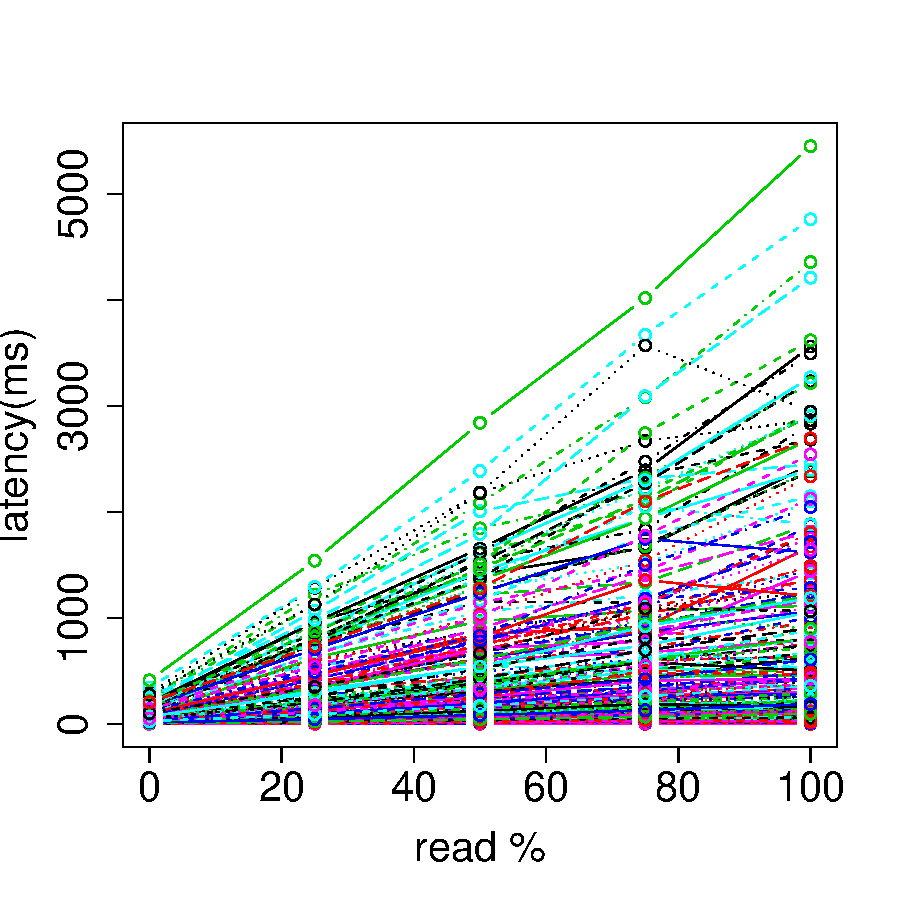
\includegraphics[width=0.5\textwidth]{figure/emc-3disk-raid0_basic_8_120s_read_single_var.pdf}}
\subfloat[N2]{\label{fig:N2read}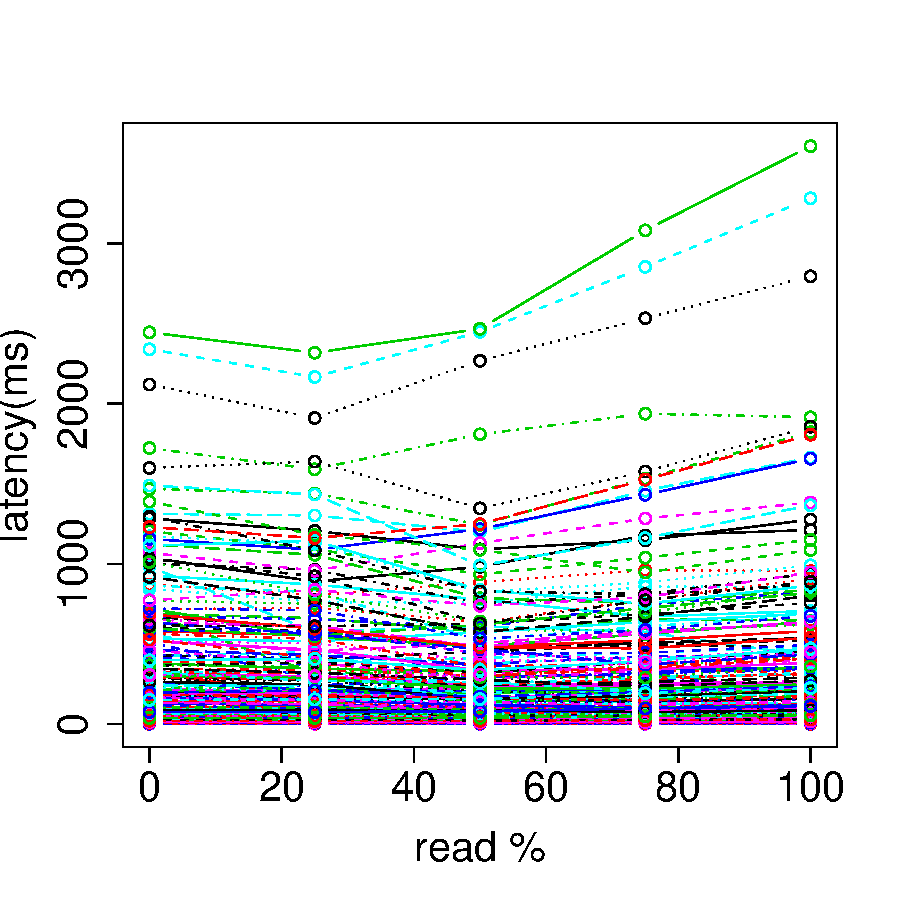
\includegraphics[width=0.5\textwidth]{figure/srs7diskfc_netapp_basic_8_120s_read_single_var.pdf}}
\captionsetup{format=myformat}
\caption{Effect of \emph{read\%} variation on the \emph{latency} of E1 and N2 data stores.
Each line represent latency~($P$) vs. read\%~($\READ$) while other parameters($\OIO$, $\SIZE$ and $\RAND$) are fixed.
The effect of $\READ$ on E1 is much more predictable(therefore significant) than N2.
}
\label{readParam}
\end{figure}
\begin{table}[!t]
\centering
\begin{tabularx}{0.9\textwidth}{
  X|
  >{\centering} X|
  >{\centering} X|
  >{\centering} X|
  >{\centering\arraybackslash} X
}
\hline
Name    & No. of disks & RAID & Interface & Make \\
\hline
\hline
E1  & 3 & 0 & SATA & EMC \\
E2  & 6 & 5 & FC   & EMC \\
N1  & 3 & 5 & SATA & NetApp \\
N2  & 7 & 6 & FC   & NetApp \\
\hline
\end{tabularx}
\captionsetup{format=myformat}
\caption{Summary of test data stores used in Storage Performance Model testing.}
\label{ds}
\end{table}
\figurename~\ref{readParam} shows the relationship between $P$ and $\READ$ for two data stores E1 and N2 from \tablename~\ref{ds}.
The plot shows the latency change observed on two different data stores while varying $\READ$ and fixing $\RAND$, $\SIZE$ and $\OIO$.
It is clear that $\READ$ has distinct effect of E1 but not on N2.
This means that $M_W$ for E1 should contain $\READ$ but not N2.
An important thing to note is that the inclusion of $\READ$ in $M_W$ for N2 will result in over-fitting since it is likely to only add to the noise.
Therefore, removing $\READ$ from the workload model actually results in a more robust model that is less sensitive to noise.

Another difficulty arises from the fact that the interactions between the characteristics are significant and cannot be ignored.
While it is possible to use a simple tuple of $\RAND$, $\READ$, $\SIZE$ and $\OIO$, we found the resulting $\epsilon$ to be very large.
Interactions between the characteristics can be factored in by simply adding additional terms for the products of two or more characteristics.
For example, the interaction between $\RAND$ and $\READ$ can be factored in to the model by adding the additional term $\RAND:\READ = \RAND*\READ$.
Therefore, given 4 characteristics, there are $2^4-1=15$ possible terms including the interactions.
To check which of the 15 terms actually have a significant effect on the performance, we conduct ANOVA at 95\% confidence controlling the 15 terms~(using the test vector) and observing the latency on four test data store shown in \tablename~\ref{ds}.

\begin{table}[!t]
\centering
\begin{tabularx}{0.9\textwidth}{
  X|
  >{\centering}X||
  X|
  >{\centering\arraybackslash}X}
\hline
\multicolumn{2}{c||}{E1}  & \multicolumn{2}{c}{E2} \\
\hline
factor        & p-value & factor        & p-value     \\
\hline
\OIO          & 4.83e-06  & \OIO          & $<$ 2e-16   \\
\READ:\OIO        & 3.09e-08  & \RAND:\OIO      & 7.92e-15    \\
\SIZE:\OIO        & 3.45e-03  & \SIZE:\OIO        & $<$ 2e-16   \\
\RAND:\READ:\OIO    & $<$ 2e-16 & \RAND:\READ:\OIO    & $<$ 2e-16   \\
\RAND:\SIZE:\OIO    & 4.51e-03  & \RAND:\SIZE:\OIO    & 3.98e-05    \\
\RAND:\READ:\SIZE:\OIO  & 5.99e-11  & & \\
\hline\hline
\multicolumn{2}{c||}{N1}  & \multicolumn{2}{c}{N2}  \\
\hline
factor        & p-value & factor        & p-value     \\
\hline
\OIO              & 6.85e-03  & \OIO          & 3.06e-16      \\
\RAND:\OIO            & $<$ 2e-16 & \RAND:\OIO        & $<$ 2e-16     \\
\SIZE:\OIO            & $<$ 2e-16 & \SIZE:\OIO        & $<$ 2e-16     \\
\RAND:\READ:\OIO          & 2.33e-05  & \RAND:\READ:\OIO      & 4.68e-08      \\
\RAND:\SIZE:\OIO          & $<$ 2e-16 & \RAND:\READ:\SIZE:\OIO    &   $<$ 2e-16   \\
\RAND:\READ:\SIZE:\OIO        & $<$ 2e-16 &           & \\
\hline
\end{tabularx}
\captionsetup{format=myformat}
\caption{Result of factorial ANOVA with latency as response and characteristics of workload as the treatment.
Only the factors with p-values less than 0.05 are shown.
With 95\% probability, these factors have a predictable effect on performance.
}
\label{p_values}
\end{table}
The \emph{p-values} derived from the ANOVA test is shown in \tablename~\ref{p_values}.
These values have a significant effect on performance~($P$) with 95\% confidence.
For example, the $M_W$ for E2 is a row vector of the form;
\begin{equation}
M_W = \begin{bmatrix} \OIO & \RAND*\OIO & \SIZE*\OIO & \RAND*\READ*\OIO & \RAND*\SIZE*\OIO \end{bmatrix}
\end{equation}
The resulting $M_W$ accounts for any interactions as well as their significance on a given data store.
While the cost of the experiment is not cheap, this only has to be done once per data store type in the system.

\subsection{Data Store Model}
\begin{table}[!t]
\centering
\begin{tabularx}{0.9\textwidth}{
  X|
  >{\centering}X||
  X|
  >{\centering\arraybackslash}X
}
\hline
\multicolumn{2}{c||}{E1}  & \multicolumn{2}{c}{E2}    \\
\hline
factor                & coefficients  & factor            & coefficients  \\
\hline
\OIO                    & 1.064         & \OIO                & 8.370e-01     \\
\READ:\OIO              & 2.828e-02     & \RAND:\OIO        & 6.163e-03     \\
\SIZE:\OIO              & 1.505e-05     & \SIZE:\OIO          & 1.172e-05     \\
\RAND:\READ:\OIO        & 2.277e-03     & \RAND:\READ:\OIO    & 4.079e-04     \\
\RAND:\SIZE:\OIO        & 2.545e-07     & \RAND:\SIZE:\OIO    & 9.970e-08   \\
\RAND:\READ:\SIZE:\OIO  & 9.385e-09     &                   &               \\
\hline\hline
\multicolumn{2}{c||}{N1}  & \multicolumn{2}{c}{N2}          \\
\hline
factor                & coefficients  & factor                & coefficients\\
\hline
\OIO                    & 1.428         & \OIO                    & 1.310\\
\RAND:\OIO            & 1.653e-01     & \RAND:\OIO            & 1.403e-01\\
\SIZE:\OIO              & 1.293e-04     & \SIZE:\OIO              & 9.078e-05\\
\RAND:\READ:\OIO        & -3.24e-04   & \RAND:\READ:\OIO        & 1.579e-06\\
\RAND:\SIZE:\OIO        & 2.052e-06     & \RAND:\READ:\SIZE:\OIO  & 1.514e-08\\
\RAND:\READ:\SIZE:\OIO  & 2.613e-08     &                       & \\
\hline
\end{tabularx}
\captionsetup{format=myformat}
\caption{Data store model~($M_S$) for four test data stores.
~($M_S$) is a column vector whose entries are shown in the \emph{coefficients} column of the each data store.}
\label{smodel}
\end{table}

Using the $M_W$, we find the $M_S$ using Equation~\ref{msSolve}.
\tablename~\ref{smodel} shows the resulting $M_S$ for the four test data stores.
The \emph{coefficients} columns of each data store form a column vector which is $M_S$ of that data store.
The accuracy of $M_S$ depends heavily on the number of data points.
While initially it can be derived from our test vector, it can be updated from the data collected in production environment to improve its accuracy.
%A great thing about linear regression is that it can also provide a \emph{prediction interval} based on the observed error distribution.

\subsection{Performance Model}
Finally, we are now ready to calculate $M_P$, which is the prediction of $P$, by taking the cross product of $M_S$ and $M_W$.
One interesting thing to note from \tablename~\ref{p_values} is that all the factors contain $\OIO$.
This is because the average latency~($P$) of all data stores are linear to the number of outstanding IOs~($\OIO$).
Note that it also means that $P$ is not linear to $\RAND$, $\READ$ and $\SIZE$.

We have tested 12 different data stores and verified that the linear relationship between the outstanding IOs and the latencies hold.
%Let us denote the element of $M_S$ that corresponds to an element of $M_W$ as $M_{S,W}$.
%For example, $M_{S=E1,\OIO}=1.064$ which is the coefficient corresponding to $\OIO$ in \tablename~\ref{smodel} for data store E1.
Therefore, we can rewrite Equation~\ref{msSolve} as;
\begin{equation}\label{rpm:eq}
\begin{split}
M_P&=M_WM_S=M_W'M_S\OIO\\
M_W'&=\frac{M_W}{\OIO}
\end{split}
\end{equation}

Since the \emph{outstanding IO}~($\OIO$) is the number of IO requests outstanding in the queue and $P$ is time the requests spend in the system, by Little's law~\cite{little:1961}, $M_W'M_S$ is the average inter-arrival time of requests.
It is also the average service time of requests at equilibrium and its inverse is the throughput~($T$) in $\mathit{IO}/s$.
Pesto~\cite{gulati:2011} describes the linear relationship between $\OIO$ and $P$ in much more depth and we refer interested readers to their work.

\begin{figure}[!t]
\centering
\subfloat[E1]{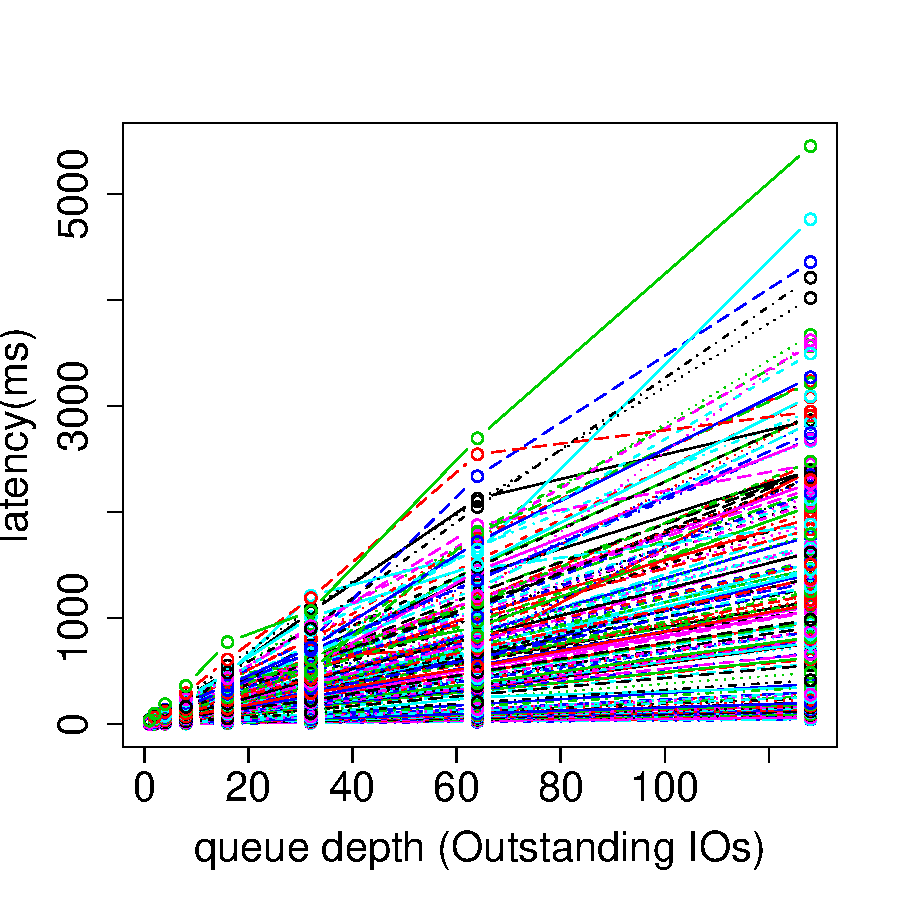
\includegraphics[width=0.5\textwidth]{figure/emc-3disk-raid0_basic_8_120s_oio_single_var.pdf}}
\subfloat[E2]{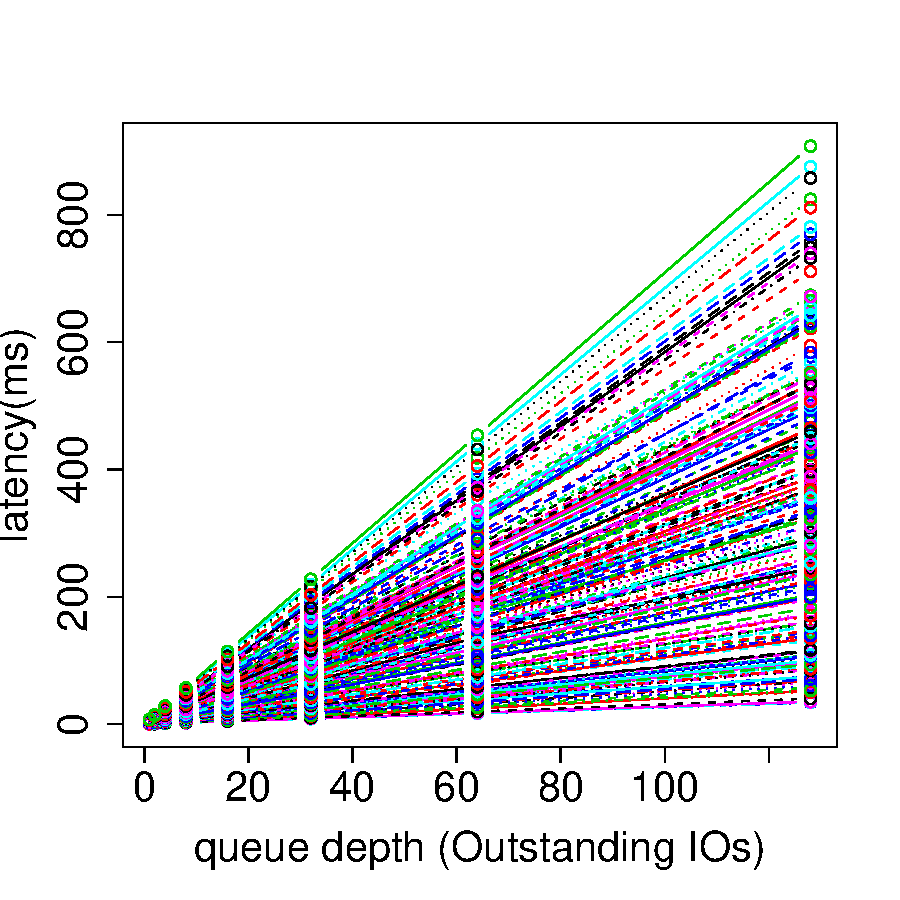
\includegraphics[width=0.5\textwidth]{figure/emc-6diskfc-sp_basic_8_120s_oio_single_var.pdf}}\\
\subfloat[N1]{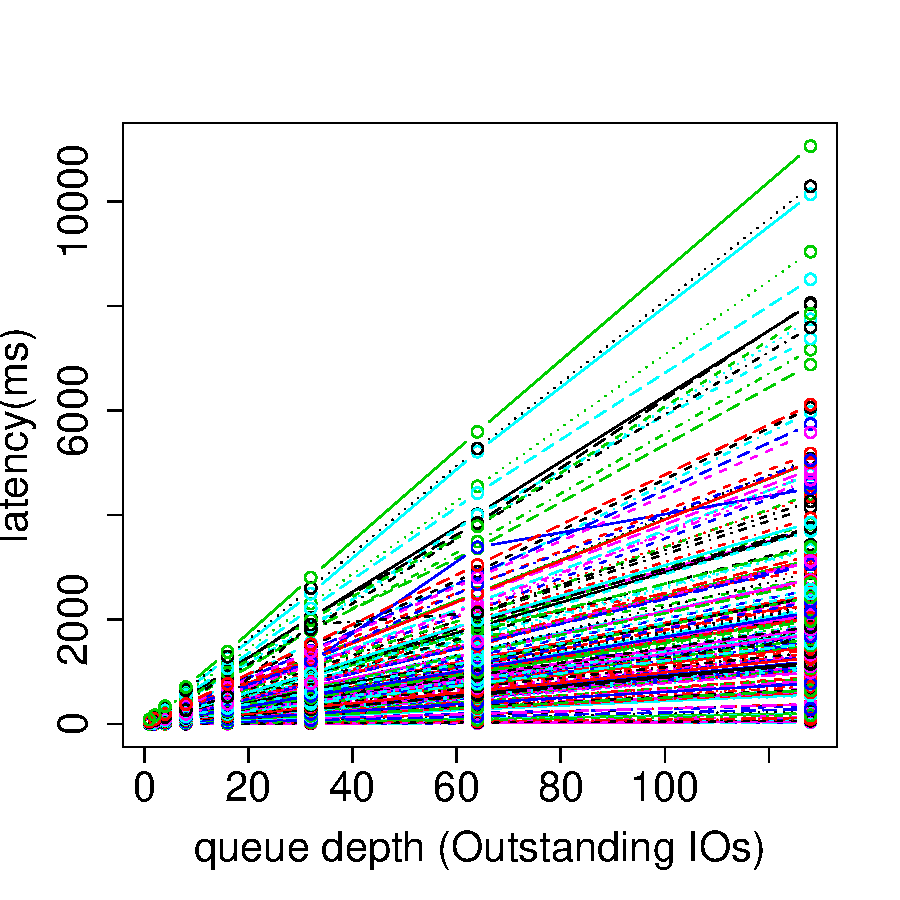
\includegraphics[width=0.5\textwidth]{figure/netapp-3diskata-sp_basic_8_120s_oio_single_var.pdf}}
\subfloat[N2]{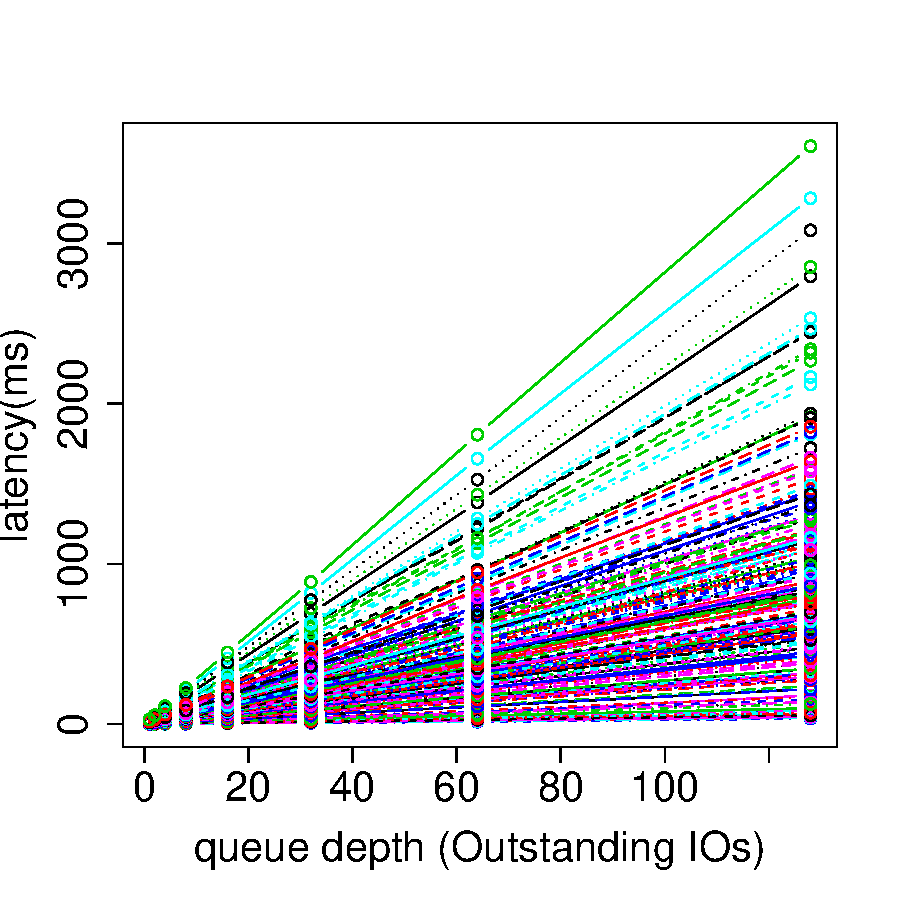
\includegraphics[width=0.5\textwidth]{figure/srs7diskfc_netapp_basic_8_120s_oio_single_var.pdf}}
\captionsetup{format=myformat}
\caption{Effect of outstanding IO~($\OIO$) variation~(from 1 to 128) on the latency of test data stores.
Each line represent latency~($P$) vs. outstanding IO~($\OIO$) while other parameters are fixed.
Except for the few noise, the relationship is clearly linear for all data stores.
}
\label{oioParam}
\end{figure}
%Simply put, $M_W'M_S'$ is the rate at which the latency increases as more IOs are outstanding at the queue which is constant for all data stores as shown in \figurename~\ref{oioParam}.
The \figurename~\ref{oioParam} shows latency~($P$) change as $\OIO$ is varied while fixing $\RAND$, $\READ$ and $\SIZE$.
Except for some exceptions caused by the measurement errors, all plots show linear relationship between $\OIO$ and $P$.
%Some exceptions are shown which we believe are caused by measurement errors.
$M_W'M_S$ is called \emph{LQ-slope} in Pesto, and we continue to use the terminology for the sake of consistency.
Therefore, we can rewrite Equation~\ref{rpm:eq} to our final form of $M_P$.
\begin{equation}\label{rpmf:eq}
P=M_P+\epsilon=\mathit{LQslope}*\OIO+\epsilon=M_W'M_S\OIO+\epsilon
\end{equation}
There are two benefits of using Equation~\ref{rpmf:eq} compared with Equation~\ref{rlm}.
First benefit is that $\OIO$ no longer needs to be modeled.
This effectively reduces the size of $M_S$ and $M_W$ simplifying the modeling process as well as prediction process.
The second benefit comes when we derive the \emph{Workload Aggregation Model} which we will describe in \CHP~\ref{ROMANO}.

\subsection{Prediction Interval}
The most important feature of our model is that it provides the confidence of its own prediction.
The model keeps track of the variance~($\sigma^2$) of $\epsilon$ from which the prediction interval is calculated to be;
\begin{equation}\label{ci}
M_P\pm\frac{1.96\sigma}{\sqrt{n}}
\end{equation}
at 95\% confidence.
Therefore, the 95\% of actual $P$ should fall within the confidence interval.
$n$ is the number of data points and $\pm1.96\sigma$ is used to capture the 95\% of the Gaussian distribution which we assume is the distribution of $\epsilon$.
In short, the prediction interval is proportional to the variance of residuals and inversely proportional to the square root of the number of observations.
If the prediction interval is too large, the prediction is useless.
To tighten the interval we can do two things.
First is to reduce the confidence level.
However this approach may lead to too many bad predictions that could result in bad decision making.
Another approach is to increase the number of observations.
In our model, the performance statistics and the workload characteristics are collected in real time to update the $M_S$ in effort to tighten the prediction interval.

\subsection{Stats Collector}
In order to update $M_S$, the \emph{stats collector} collects workload characteristics and performance in real time.
$P$ is measured at vSCSI layer as the completion time subtracted from time of queueing per request.
$\READ$ and $\SIZE$ are simply read from IO request attributes.
$\OIO$ is measured from the queue depth of the \emph{vSCSI}~\cite{ahmad:2011} device which is created per virtual machine~(VM) and virtualizes the SCSI device layer.
%To facilitate the \emph{stats collection}(step 2) of \figurename~\ref{rpm}, $\RAND$ must also be collected.
We had to implement the mechanism to collect $\RAND$ at SCSI device layer since vSCSI is unaware of large seeks that result from seeking between multiple virtual disks in a data store.
$\RAND$ is measured by simply looking at the percentage of seeks larger than 10 times the average request size.
The reason for the multiplier is that some workloads exhibit significant variance in their request size. Since the seeks are measured in terms of address difference between consecutive requests, large requests could falsely register as seeks even when they are sequential.
All stats are averaged and reported to \emph{Resource Manager} at 20 seconds granularity.

\section{Prediction Accuracy}

\begin{table}[!t]
\centering
%\begin{tabular}[t]{l|S S S S}
\begin{tabularx}{0.9\textwidth}{
  X|
  >{\centering} X|
  >{\centering} X|
  >{\centering} X|
  >{\centering\arraybackslash} X
}
\hline
          & Basil     & Pesto     & FFLM        & Proposed      \\
\hline
\hline
Min.      & -27380    & -1.33     & -1669       & -1667   \\
1st Qu.   & -441.8    & 12.03     & -0.1037     & -8.610    \\
Median    & -105.2    & 52.67     & -0.7699     & -0.1033     \\
Mean      & -565.6    & 292.5     & 1.860e-13   & 1.191     \\
$|$Mean$|$& 642.4     & 292.5     & 44.43       & 44.34   \\
3rd Qu.   & -22.31    & 243.8     & 7.872       & 9.043     \\
Max.      & 6242      & 10590     & 1141        & 1146        \\
\hline
\end{tabularx}
\captionsetup{format=myformat}
\caption {Comparison of residuals ($\epsilon$) for different modeling techniques.
The residuals were aggregated from all four data store models.
1st Qu. and 2nd Qu. represents 25\% and 75\% quantile values respectively.
$|$Mean$|$ represents mean of absolute values of residuals.
Units are in $\mathit{ms}$.}
\label{residualsAll}
\end{table}

This section evaluates the accuracy and the robustness of our performance model.
Specifically, we use Basil~\cite{gulati:2010} and Pesto~\cite{gulati:2011} as the baseline models and assume that the \emph{full factorial linear model} (FFLM) is the ideal case since it uses all possible linear combinations.
To evaluate the accuracy we use \emph{test vector} and run them against for 4 test data stores (\tablename~\ref{ds}).
The resulting 6400 latencies are compared against the predictions of 4 techniques.

\tablename~\ref{residualsAll} shows aggregated $\epsilon$ values, the difference between the prediction ($M_P$) and the measurements ($P$), of different modeling techniques.
The values were aggregated from latency prediction of all four data stores under test (from 6400 data points).
It shows that the performance of Basil is unacceptable in a heterogeneous data store environment for most applications with high mean $\epsilon$ of $642\mathit{ms}$.
This is expected since Basil generates a single model for any data stores.
Pesto takes into the account the performance difference of each data store.
However, it assumes that one data store is simply more powerful than the other regardless of the workload.
While it provides a better accuracy than Basil by 60\% on average, it still shows unreasonable maximum $\epsilon$ of $10s$ and average $\epsilon$ of $260\mathit{ms}$.

Our proposed model shows a much stronger predictive power with average $\epsilon$ of $44\mathit{ms}$ and the maximum $\epsilon$ of $1.3s$.
This is an 82\% reduction for the maximum residual and 83\% reduction for the average residual compared to Pesto.
In fact, our model performs slightly better than FFLM although the difference is too small to be meaningful.
However, this model is capable of faster model updates and prediction since it only uses 4-5 terms versus 16 terms used by FFLM.
Furthermore, 50\% of all predictions (between the 1st and 3rd quantile) exhibit less than $10\mathit{ms}$ of error.

In short, our proposed model shows 80\% improvement in overall prediction accuracy on heterogeneous workloads and data stores compared to the most recent technique~\cite{gulati:2011}.
%The performance can be improved by using piecewise linear regression techniques and filtering mechanisms by 19\% and 44\% on average respectively.
%While the piecewise linear regression techniques offer better reduction of maximum residual, filtering mechanism provides better reduction of average residual.
%Furthermore, filtering mechanism has lower prediction overhead since you still need only a single model for each data store.
%The usefulness of these techniques are still being evaluated and are left for our future work.

\section{Prediction Interval}
\begin{figure}[!t]
\centering
\includegraphics[width=0.8\columnwidth, clip, trim=0 0.2in 0 0.7in]{figure/prediction_interval2.pdf}
\captionsetup{format=myformat}
\caption{The average latency (over 20 second intervals) observed from
  20 different workloads (running on separate virtual disks) on 4
  different test data stores during 1 hour interval.  The max and min
  latency is plotted. Also plotted are the model's 95\% prediction
  intervals.}
\label{predInterval}
\end{figure}

Perhaps the most significant benefit of our model is its ability to provide a prediction interval at pre-defined confidence for its predictions.
\figurename~\ref{predInterval} shows the average latencies of 20 different virtual disks running different workloads randomly selected from our test vector on four test data stores.
The average was evaluated over two minutes.
The predicted latency and its corresponding interval (shown as the error bar)  was calculated using our model at 95\% confidence (allowing 5\% of measurements to be outside of the prediction interval).

\figurename~\ref{predInterval} shows that the predictions can be off by up to $500\mathit{ms}$ (\emph{workload 16}).
However, all measurements fall within the prediction interval.
In fact, out of 1600 workloads ran against 4 data stores in the previous experiment, our model failed to capture the measured latency within its prediction interval 423 times which is 6.6\% (close to predefined 5\%) of 6400 predictions made.

Another interesting thing is that there were roughly 5\% of workloads whose confidence interval is so large, like the \emph{workload 6} in \figurename~\ref{predInterval}, that the prediction itself is meaningless.
Pesto~\cite{gulati:2011} claimed that these workloads had specific characteristics (such as purely sequential) and can be filtered out.
However, we found them to be more of random occurrences and difficult to predict in advance.
By default, the prediction is done every 8 hours to consider the possible moves in current VMware products~\cite{epping:2011}.
However, we force prediction every 2 minutes and observed prediction interval change after 5 hours.
In theory, the prediction interval should converge after about 2 hours (12 measurements), however we found the convergence to take a much longer time.
We suspect the reason to be fluctuation in the workload.
A detailed analysis and speeding up this convergence will be our future work.

In short, our model is capable of providing prediction interval at a specified confidence level.
The level of confidence can be lowered to trigger more aggressive load balancing with tighter prediction interval.
On the other hand a higher confidence interval will result in moves that are only triggered when predicted benefit is large enough to over come the larger prediction interval.

\section{Handling Heterogeneous Data Stores}

\begin{figure}[!t]
\centering
\subfloat[Measured Relative Latency]{\label{slm}\includegraphics[width=0.7\textwidth, clip, trim=0 0.2in 0in 0.5in]{figure/sorted_latency.pdf}}\\
\subfloat[Pesto Prediction - relative]{\label{slp}\includegraphics[width=0.7\textwidth, clip, trim=0 0.2in 0in 0.5in]{figure/pesto_sorted_latency.pdf}}\\
\end{figure}
\begin{figure}[!t]
\ContinuedFloat
\centering
\subfloat[Our Prediction - relative]{\label{slr}\includegraphics[width=0.7\textwidth, clip, trim=0 0.2in 0in 0.5in]{figure/romano_sorted_latency.pdf}}
\captionsetup{format=myformat}
\caption{Sorted normalized latency plot for four test data stores.
It shows the relative latencies of E1, N1 and N2 compared to E2.
The 1600 latencies measured from each data store were normalized by E2 and than sorted.
The y-axis represents the normalized latency and the x-axis represents the sorted index.
The actual measurements as well as predictions from Pesto and our model are plotted.
Pesto assumes a linear performance difference between the workloads so there is only a linear difference between the data stores regardless of the workloads.
For the actual measurement, all four lines cross each other, suggesting that data stores are seldom slower than the other data store for all workloads.
While Romano does not capture this effect fully, it does capture the most distinct features of real measurements.
}
\label{sortedLatency}
\end{figure}

In this section, we evaluate the model's ability to handle heterogeneous data stores using Pesto~\cite{gulati:2011} as the baseline.
Basil is not compared here since it only generates a single model across the data stores and can not handle heterogeneity.
Pesto injects a \emph{4KB, random and read-only} workload into the data store to derive the \emph{LQ-slope} for a given data store.
\tablename~\ref{pestolq} shows the Pesto LQ-slope of four test data stores.
Since each data store has a fixed LQ-slope regardless of the workload, running same workloads on multiple data stores will always result in constant ratio equal to the LQ-slope ratio.
\begin{table}[!t]
\centering
\begin{tabularx}{0.9\textwidth}{
  >{\centering}X|
  >{\centering}X|
  >{\centering}X|
  >{\centering\arraybackslash}X
}
\hline
E1          &   E2      &   N1      &   N2 \\
\hline
\hline
25.798101   & 4.922433  & 16.666000 & 6.753044 \\
\hline
\end{tabularx}
\captionsetup{format=myformat}
\caption{Pesto LQ-slope of four test data stores.  The units are
  $\mathit{ms/io}$.  According to these slopes, E2 is the fastest data
  store and E1 is the slowest.}
\label{pestolq}
\end{table}
\figurename~\ref{slp} plots this effect.

\figurename~\ref{slm} shows the latency normalized by E2 latencies from running our \emph{test vector}.
As expected, most of latencies observed in other data stores are larger than that of E2 (with the smallest LQ-slope hence the fastest) but surprisingly, there exist some corner cases where even the slowest E1 out performs E2.
In fact, N1 seems to have the highest latency of all data stores on average even though its LQ-slope is lower than E1.
\figurename~\ref{slr} shows that our model is able to capture this relative difference fairly accurately.
For those corner cases where the model fails to capture the exact relative order of performance, the prediction intervals tend to be very large.
Therefore, Romano will not make any predictions for those cases with high confidence indicating that actions should not be made based on the prediction values only.

\begin{figure}[!t]
\centering
\subfloat[Pesto]{\label{rdPesto}\includegraphics[width=0.6\textwidth, clip, trim=0 0.2in 0in 0.7in]{figure/error_hist_compare_pesto.pdf}}\\
\subfloat[Proposed model]{\label{rdRomano}\includegraphics[width=0.6\textwidth, clip, trim=0 0in 0.2in 0.7in]{figure/error_hist_compare_kromano.pdf}}
\captionsetup{format=myformat}
\caption{Distribution of residuals ($\epsilon$) for Pesto and Romano.
x-axis is the value of $\epsilon$ in $ms$.
y-axis is number of occurrences+1.
Addition of 1 was required to allow y-axis to be in log scale.
}
\label{residualDist}
\end{figure}
\figurename~\ref{rdPesto} shows that the residual ($\epsilon$) distribution of Pesto varies widely depending on the data store.
The accuracy of Pesto on a single data store provides little information about how it might do on another data store.
As the new data stores are introduced into the storage pool, the applicability of Pesto needs to be re-evaluated.

On the other hand, our model shows a much more even distribution across the data stores in \figurename~\ref{rdRomano}.
While there are some differences, prediction accuracy of our model is robust against the heterogeneity of data stores.
Furthermore, the model's prediction interval further improves its robustness by generating larger interval for the data stores that are difficult to model.
In short, proposed technique provides robust and adaptive models across the heterogeneous data stores with a single framework.
